\documentclass{article}

\usepackage{amsmath}
\usepackage{pgfplots}
\graphicspath{ {./images/} }
\usepackage{ragged2e}
\usepackage{blindtext}

\title{Introduccion a Series Temporales - Conceptos y Metodología}
\author{Javier Contreras}
\date{\today}



\begin{document}

	\maketitle
	\section{Componentes de las Series Temporales}
        Pongamos la siguiente serie temporal:
	\begin{figure}[h]
		\centering
                \label{fig_1}
                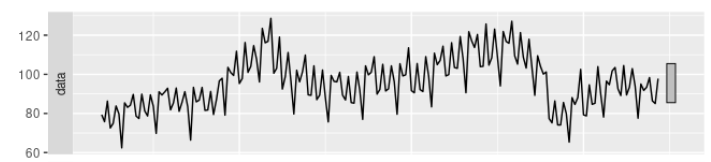
\includegraphics[width=10cm]{Ejemplo_Serie_Temporal}
		\caption{Serie Temporal - Datos en crudo}
	\end{figure}
Se puede descomponer en una señal de \textbf{Estacionalidad}, una señal de \textbf{Tendencia-Ciclo} y la señar restante, llamada \textbf{Residuo}. \\

Esta descomposición se puede realizar de dos maneras, la primera es la descomoposición Aditiva y la segunda se llama descomposición Multiplicativa.\\
La descomposicion aditiva es la más apropiada si la magnitud de las fluctuaciones estacionales, o la variacion de la tendencia-ciclo, no varía en funcion del \textit{nivel} de la serie temporal. 
        Cuando la variación en el patrón estacional o en la tendencia es proporcional al \textit{nivel} de la serie temporal, entonces la descomposición multiplicativa es más apropiada.\\
        \begin{itemize}
                \item \textbf{Descomposición Aditiva} $y_{t} = S_{t} + T_{t} + R_{t}$\\
                \item \textbf{Descomposición Multiplicativa} $y_{t} = S_{t} \times T_{t} \times R_{t}$
        \end{itemize}

\newpage



Descomponiendo la señal de la figura 1 de manera aditiva, podemos obtener las siguientes señales:

	\begin{figure}[h]
		\centering
                \label{fig_2}
                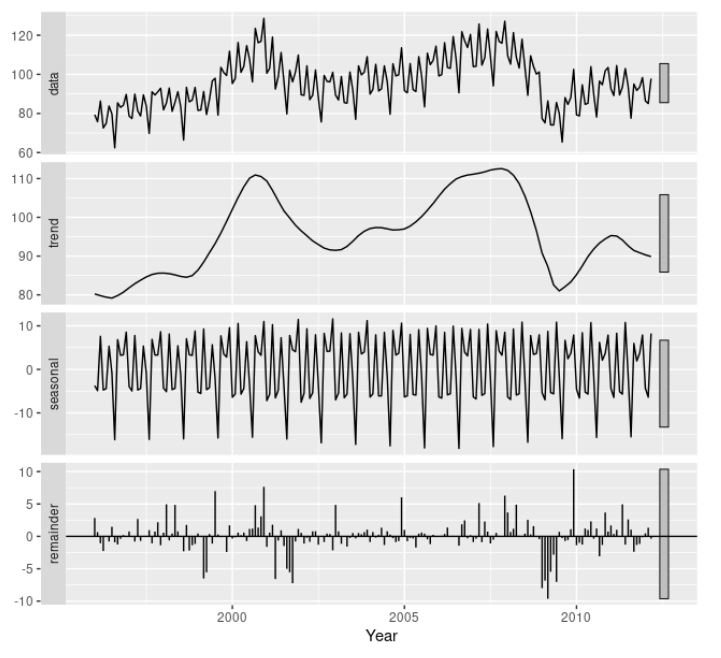
\includegraphics[width=10cm]{Ejemplo_ST_descomposicion}
		\caption{Serie Temporal - Descomposición Aditiva}
	\end{figure} 
        El algunos casos puede resultar beneficioso quitar la componente estacional de la señal, por ejemplo en estudios sobre la variación del desempleo.


        \section{Medias en movimiento}

        El método clásico de estimacón de Tendencias-Ciclos es el de las medias en movimiento.
        
        \begin{equation}
                \label{eq_1}
                \hat{T}_{t} = \frac{1}{m}\displaystyle\sum_{j=-k}^{k}y_{t+j}
        \end{equation}

        Donde $m = 2K +1$. La estimacion de la tendenci-ciclo en \textit{t} se obtiene realizando la media de los valores entre los \textit{k} periodos de \textit{t}. La notacion es del tipo m-MA, donde el valor a elegir es k. Cuanto más alto, más plana será la tendencia. Normalmente se usan números impares para \textit{k}.
        \newpage

        En algunos casos se aplica el método de medias en movimiento a las medias en movimiento de una serie temporal. Esto se usa, por ejemplo, para estimar la tendencia-ciclo con datos estacionales, también se usa para obtener resultados simétricos. Se denotaria por ejemplo como $2 \times $4-MA:


        \begin{equation}
                \label{eq_2}
                \hat{T}_{t} = \frac{1}{8}y_{t-2}+\frac{1}{4}y_{t-1}+\frac{1}{4}y_{t}+\frac{1}{4}y_{t+1}+\frac{1}{8}y_{t+2}
        \end{equation}
        
        En este caso se podría aplicar a una serie temporal cuaternaria, en la que el primer elemento y el último corresponden al mismo periodo estacional, teniendo el mismo peso.\\

        Si el periodo estacional es par, entonces se usará $2 \times$ \textit{m}-MA. Si, sin embargo, el periodo estacional es impar, se usará \textit{m}-MA. De esta forma, $2 \times$ 12-MA se usará para estimar tendencias-ciclos de datos con estacionalidad mensual. 7-MA se usará para estimar tendencias-ciclos en datos con estacionalidad semanal.\\

        Las combinaciones de medias en movimiento son equivalentes a aplicar medias en movimiento con pesos. Así, $2 \times$ 4-MA es equivalete a 5-MA con pesos [$ \frac{1}{8},\frac{1}{4},\frac{1}{4},\frac{1}{4},\frac{1}{8}$]. En general, un \textit{m}-MA puede escribirse como:
        \begin{equation}
                \label{eq_}
                \hat{T}_{t} = \displaystyle\sum_{j=-k}^{k}a_{j}y_{t+j},
        \end{equation}
        donde $k = (m-1)/2$ y los pesos dados por $a_{j}$ son simétricos y suman 1. En realidad, \textit{m}-MA es solo una particularizacion donde los pesos valen 1/\textit{m}.\newline

        Una ventaja de usar medias en movimiento con pesos es que dan lugar a tendencias-ciclos suavizados. En vez de entrar con el mismo peso las observaciones, estas entran con poco pesos y van creciendo a medida que se acercan a \textit{t} para decrecer a medida que se alejan.

        \section{Métodos de descomposición}
        Nos encontamos ahora con diferentes métodos de descomposición de series temporales. 
        \subsection{Descomposición Clásica}
        Método originado alrededor de 1920. Ampliamente usado aunque no se trata del método más preciso.\newline
	\begin{figure}[h]
		\centering
                \label{fig_3}
                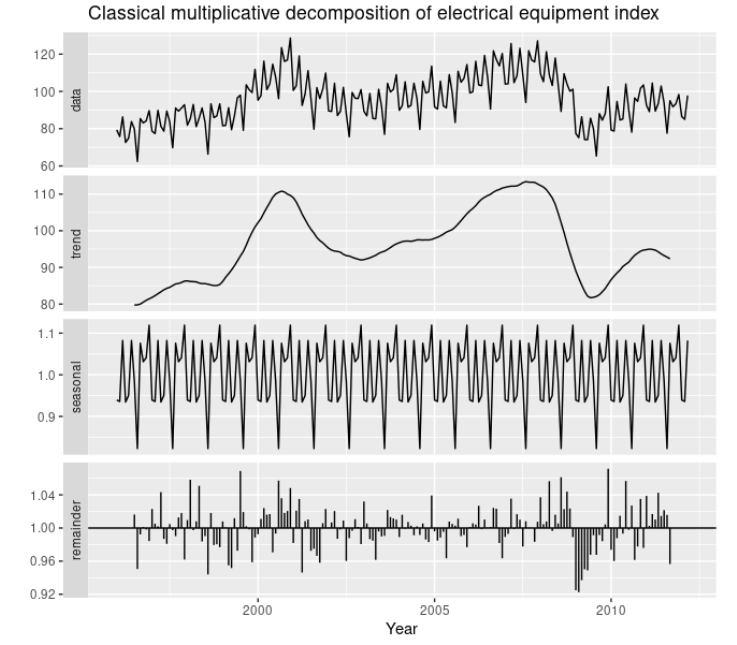
\includegraphics[width=10cm]{Ejemplo_descomposicion_clasico}
		\caption{Serie Temporal - Descomposición Multiplicativa - Método Clásico}
	\end{figure} 
        
        El ejemplo de \ref{fig_3} muestra una descomposición multiplicativa en la que se puede observar cómo se ha filtrado una bajada repentina de la curva en el año 2009. Esta bajada debería verse reflejada en la curva de tendencia y no en la curva residual.
        
        Por otro lado, los primeros valores y los últimos, no pueden ser incluidos en lás descomposiciones.

        Además, la descomposición clásica asume que la componente estacional es constante. Esto puede ser erróneo en algunos casos. Por ejemplo, los patrones de las demandas de electricidad han cambiado en los últimos años, antes era mayor en invierno por la calefaccón, ahora es mayor en verano.

        \subsection{Descomposición X11}
        Este método está basado en la descomposición clásica, pero con múltiples pasos extra para poder corregir los inconvenientes del método primero. 
        
        Siendo posible la inclusión de cambios rápidos en la tendencia en la curva que le corresponde. Además, incluye los valores frontera de la serie en las descomposiciones y acepta ligeros cambios en la estacionalidad. \newpage
	\begin{figure}[h]
		\centering
                \label{fig_4}
                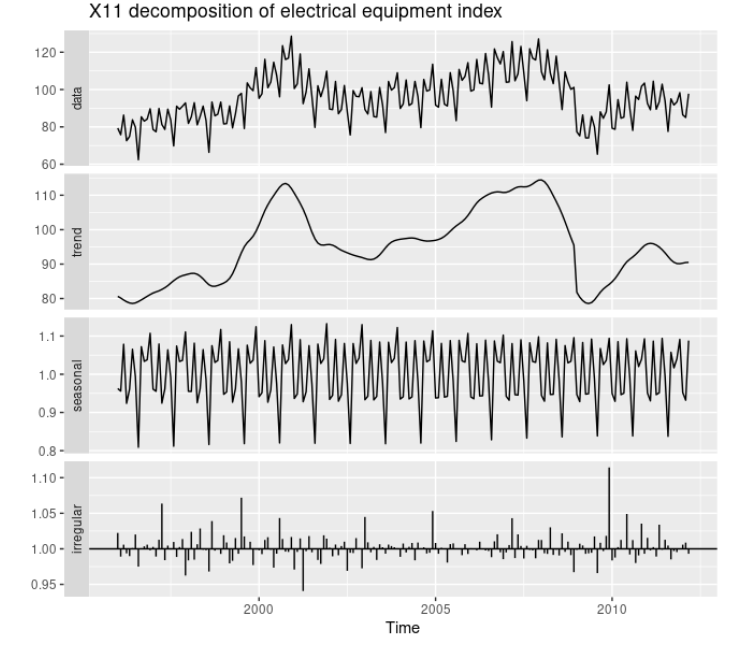
\includegraphics[width=10cm]{Ejemplo_ST_descomposicion_X11}
		\caption{Serie Temporal - Descomposición Multiplicativa - Método X11}
	\end{figure} 

        La figura \ref{fig_4} presenta la descomposición multiplicativa de la misma serie temporal que en la figura \ref{fig_3}, pero aplicando el método X11. Como se puede observar, ya no están en la señal de residuos los resultados de la tendencia decreciente rápida, estos han sido absorbidos por la curva de tendencia.

\end{document}
